\documentclass[review]{elsarticle}

\usepackage{lineno,hyperref,amsmath,amsfonts,subcaption}
\modulolinenumbers[5]

\journal{Spatial Statistics}

%%%%%%%%%%%%%%%%%%%%%%%
%% Elsevier bibliography styles
%%%%%%%%%%%%%%%%%%%%%%%
%% To change the style, put a % in front of the second line of the current style and
%% remove the % from the second line of the style you would like to use.
%%%%%%%%%%%%%%%%%%%%%%%

%% Numbered
%\bibliographystyle{model1-num-names}

%% Numbered without titles
%\bibliographystyle{model1a-num-names}

%% Harvard
\bibliographystyle{model2-names.bst}\biboptions{authoryear}

%% Vancouver numbered
%\usepackage{numcompress}\bibliographystyle{model3-num-names}

%% Vancouver name/year
%\usepackage{numcompress}\bibliographystyle{model4-names}\biboptions{authoryear}

%% APA style
%\bibliographystyle{model5-names}\biboptions{authoryear}

%% AMA style
%\usepackage{numcompress}\bibliographystyle{model6-num-names}

%% `Elsevier LaTeX' style
%\bibliographystyle{elsarticle-num}
%%%%%%%%%%%%%%%%%%%%%%%

\begin{document}

\begin{frontmatter}

\title{Spatial Log-Gaussian Cox process models and sampling paths: towards optimal design}

%% Group authors per affiliation:
\author[msuaddr]{Kenneth Flagg\corref{mycorrespondingauthor}}
\cortext[mycorrespondingauthor]{Corresponding author}
\ead{kenneth.flagg@montana.edu}

\author[msuaddr]{John Borkowski}
\author[msuaddr]{Andrew Hoegh}

\address[msuaddr]{Department of Mathematical Sciences, Montana State University, Bozeman, MT 59717}

\begin{abstract}

\paragraph{Goal of this paper (placeholder abstract---add some results when
available)} Evaluate a wide variety of path designs in terms design-based
heuristics and model-based criteria for spatial prediction using Bayesian LGCP
models. Identify promising path designs. Illuminate any relationships among
design characteristics and predictive criteria that will be helpful for
constrained optimization.

\end{abstract}

\begin{keyword}
log-Gaussian Cox process\sep optimal sampling\sep model-based design\sep spatial sampling design
%\MSC[2010] 00-01\sep  99-00
\end{keyword}

\end{frontmatter}

\linenumbers

% Can name paragraphs with \paragraph{Title}


\section{Introduction}
% State the objectives of the work and provide an adequate background, avoiding a detailed literature survey or a summary of the results.

Spatial point process models have long been considered generally infeasible
because of their computational demands, but recent advances in Bayesian
computing have made the Log-Gaussian Cox process (LGCP) an attainable model in
practice~\citep{rueetal, lindgrenetal, illianetal, simpsonetal}. In some
applications, the entire point pattern is not fully observed due to variable
sampling effort. This is referred to as a degraded point
pattern~\citep{chakrabortyetal} and it is relatively simple to accomodate
variable sampling effort in these models using modern Bayesian computing
tools~\citep{yuanetal}. However, the literature on optimal sampling for spatial
point process models is in its infancy~\citep{liuvanhatalo}.

Point pattern data are routinely collected in species distribution studies and
ordnance response projects. The data consist of the locations of event in some
spatial region. These applications may use quadrat sampling or line-transect
sampling, with transect sampling being more common. When the objective is to
map where events occur in space, various spatial mapping procedures have been
used. Traditionally these have involved aggregating the data to grid cell
counts or computing moving averages. Aggregation has the downside of
introducing arbitrary structure into the data by the choice of gridding scheme
or averaging window, and requires uneccessary computation
effort~\citep{simpsonetal}. Software is now available to fit spatial point
process models to data acquired via distance sampling and simultaneously
estimate the detection function~\citep{dspat,baser}.
% Recent example of aggregation: https://link-springer-com.proxybz.lib.montana.edu/content/pdf/10.1007/s13253-020-00386-3.pdf

In ecological settings, sampling plans are often designed around the goal of
estimating total abundance. Ordnance response surveys are typically designed
to provide enough data to detect (but not necessarily map) intensity
hotspots~\citep{em200-1-15,flaggetal}. However, to our knowledge, there has
been very little work done in deciding \emph{where} to collect data when the
goal is to map the intensity using a spatial point process model. While some
ideas about the characteristics of a good point design apply to paths, creating
an optimal path design is not as simple as connecting the points of a point
design with line segments. There are many ways to connect points into a path,
so optimal design criteria must apply to the whole path and not only to the
waypoints. In this paper, we present a variety of sampling path designs and
assess their optimality for mapping intensity using LGCP models.


\subsection{Log-Gaussian Cox process}

The log-Gaussian Cox process is an inhomogeneous Poisson process where the
logarithm of the intesity function is a Gaussian process \citep{moelleretal}.
The LGCP provides a flexible model for mapping event intensity over space using
few parameters. Efficient Bayesian computation tools available using INLA
to approximate the posterior marginal distributions \cite{rueetal}, a finite
element approach to represent the Gaussian process \cite{lindgrenetal}, and
pseudodata \cite{simpsonetal}.
% Add some example applications.


\subsection{Spatial design}

Most classical sampling and design work has been done for points or small
quadrats approximated as points, rather than paths. In two-dimensional
(geostatistical) model-based design, regularity is optimal for spatial
prediction but randomness and a variety of interpoint distances are best for
parameter estimation~\citep{diggle}. Inhibitory plus close pairs designs are a
good compromise~\citep{chipetaetal2017}. Design-based approaches exist to
spread points through high-dimensional design spaces~\citep{borkowskipiepel},
and Latin hypercube sampling has space-filling
properties~\citep{mckayetal,husslageetal}.


\subsection{Space-filling curves}

Another relevant area of research is in deterministic space-filling curves.
These have used in design of dense or stretchable
circuits~\citep{ogorzalek,mazhang} and high-dimensional data visualization
in bioinformatics~\citep{hilbertvis}. The Hilbert curve is simple to construct
and the Peano curve is very flexible for filling irregular
shapes~\citep{fanetal}. Space-filling curves are one-dimensional paths
constructed iteratively; as the number of iterations goes to infinity, the
limiting path has nonzero area and actually fills the space~\citep{sagan}. For
applications we stop after a finite number of iterations.


\subsection{Paths as sampling designs}

The small body of literature on spatial sampling design for point pattern
data has focused on line transects. \citet{pollard} began with line transcets
and adaptively added zigzags in a species abundance survey.

The Visual Sample Plan software includes features to create systamatic transect
plans and augment plans with additional transects in regions lacking spatial
coverage~\citep{vspguide}. It helps the user choose the transect spacing to
maximize the probability of detecting the presence of a hotspot of specified
size and intensity. However, it does not employ criteria to optimize spatial
prediction.

\citet{liuvanhatalo} provided one of the first explicit discussions of design
in the context of spatial LGCP models. They used narrow quadrats (swaths along
line-transects) as their sampling units. The transects were short relative to
the size of the study region and not connected into a path.


%\subsection{Multi-objective optimization}

%summarize \citet{lark} and related

%we can use a large suite of criteria to explore the relationships among them

% (Don't need for this paper.)


\section{Materials and methods}
% Provide sufficient details to allow the work to be reproduced by an independent researcher. Methods that are already published should be summarized, and indicated by a reference. If quoting directly from a previously published method, use quotation marks and also cite the source. Any modifications to existing methods should also be described.

%Kenny's heuristics of a good path design:
%\begin{itemize}
%\item Should start with a sparse design with regular spacing, then refine with
%infill
%\begin{itemize}
%\item Provides good spatial coverage even if aborted early
%\item Imagine downloading a high-resolution intensity jpeg over 56k
%\end{itemize}
%\item Path should avoid sharp turns but is allowed to cross itself
%\item One option is to generate two segments at a time, first a short-to-medium
%length segment to get to the start of the next transect, then a  medium-to-long
%segment for the transect
%\item Could have new segment length be negatively correlated with the previous
%segment length
%\end{itemize}

% Andy's words:
With an eye toward practical considerations of data collection, we present
criteria to compare sampling strategies that impact LGCP estimates. We compare
plans with (approximately) fixed path lengths, most of which avoid sharp turns.
Data collection equipment (e.g. metal detectors) may have limited mobility,
requiring minimizing the number or angle of turns. The criteria that we
evaluate are average prediction variance (APV) and mean squared prediction
error (MSPE) of the Gaussian process.


\subsection{Sampling design schemes}
\label{methodschemes}

In this section, we present three variations of parallel line transect designs
and three schemes that produce more complex designs. To clarify terminology, a
\emph{path} or \emph{design} is a realized set of one or more connected
components that has length but not area. The paths considered in this work are
constructed as sequences of line segments. A \emph{design scheme}, or simply
\emph{scheme}, is procedure for generating designs with some shared
characteristics. Figure~\ref{plancomparison} illustrates a selection of designs
from these schemes.


\subsubsection{Parallel line transects}

Parallel straight-line transects are common in ordnance response studies and in
ecological studies using distance sampling. Systematic designs are common
because they provide good spatial coverage in the sense that any point in the
study region has an a priori known maximum distance from the path. For point
designs, systematic designs are optimal for prediction, simple random samples
are optimal for estimation, and inhibitory with close pairs designs are
becoming a popular compromise. We adapt all of these to the parallel line
transect setting. We use line transects running north-south, with three ways of
choosing the horizontal coordinate: simple random sample (SRS), systematic with
a random starting point and even spacing, inhibitory plus close pairs.
Figure~\ref{plancomparison} (left column) shows an example of each scheme with
25 transects.

%We should note that we will be using an isotropic covariance function in
%the model. If an anisotropic model is used, parallel transects may need to be
%augmented with perpendicular transects so that the observed data provide the
%full range of pairwise distances in other directions.

\begin{figure}
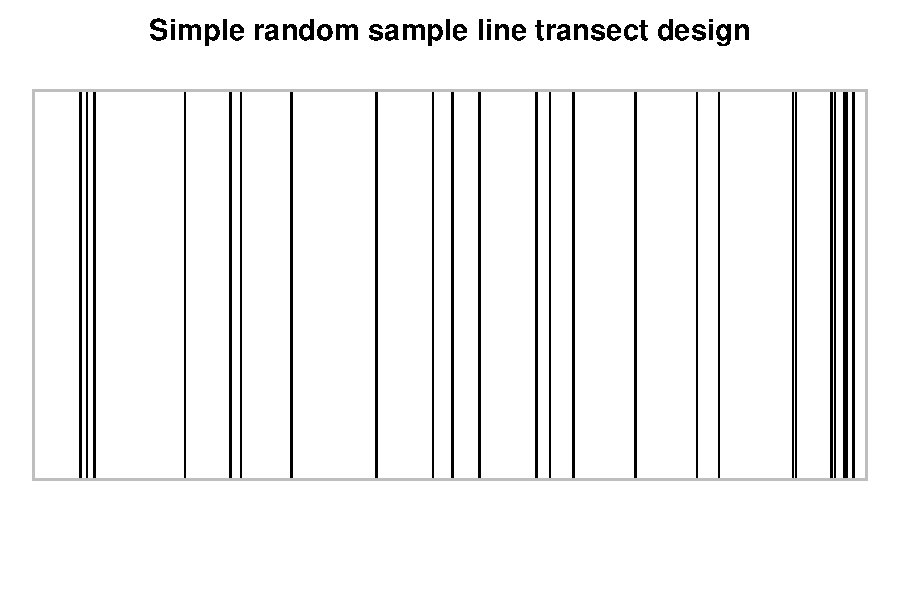
\includegraphics[width=2.5in]{SRS000176.pdf}
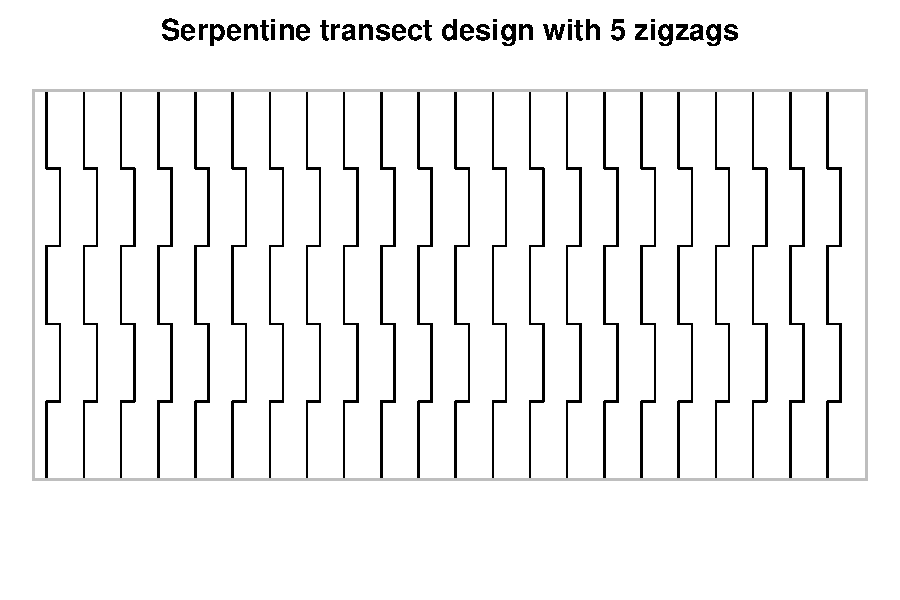
\includegraphics[width=2.5in]{Serp000124.pdf}

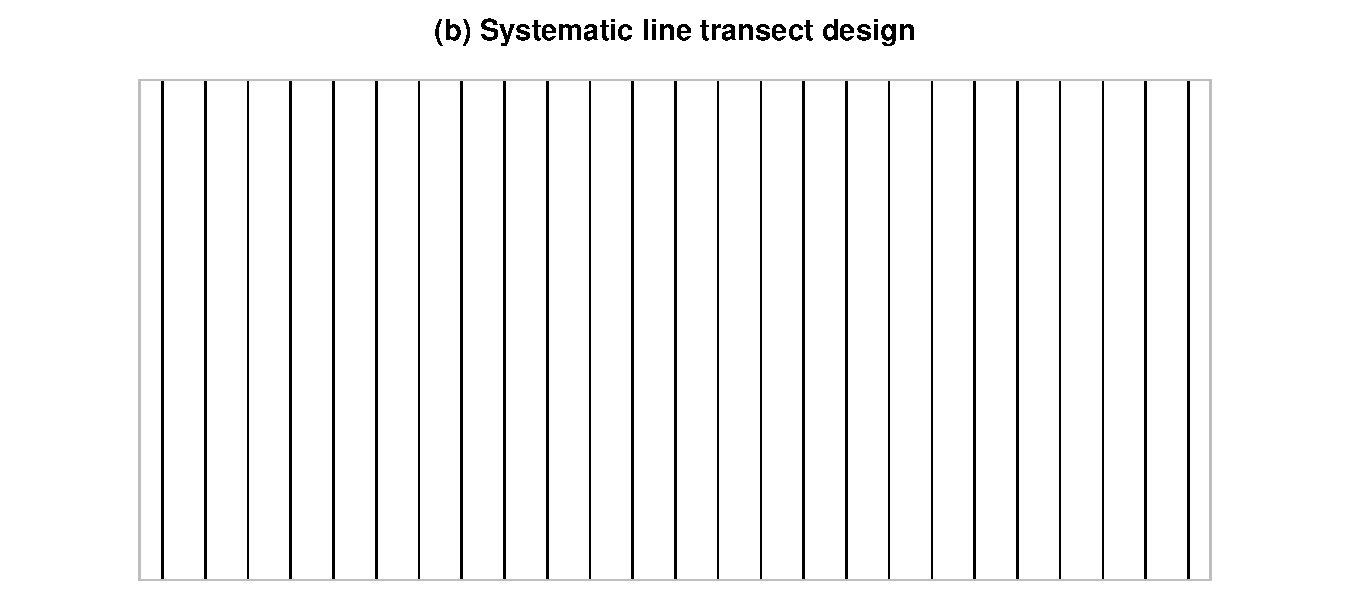
\includegraphics[width=2.5in]{Sys000141.pdf}
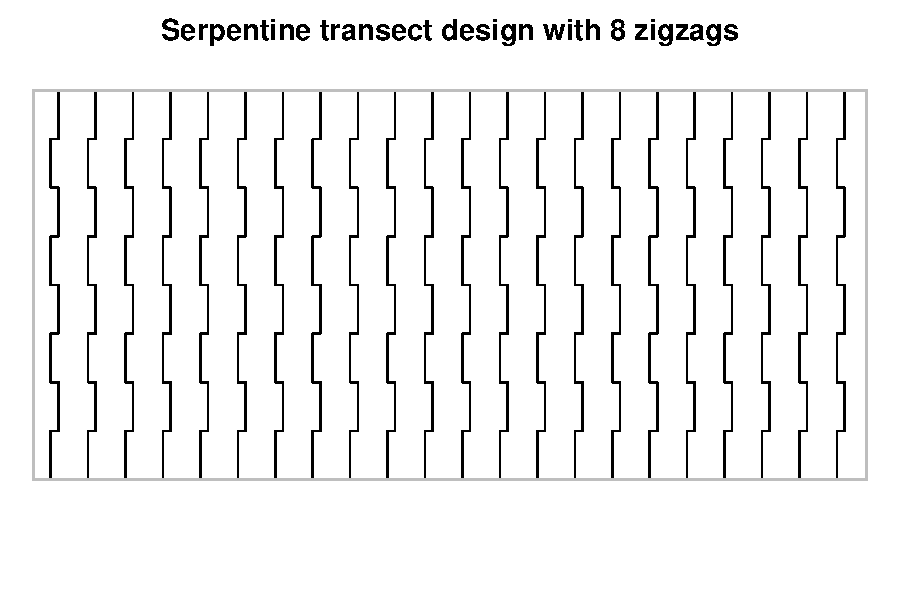
\includegraphics[width=2.5in]{Serp000539.pdf}

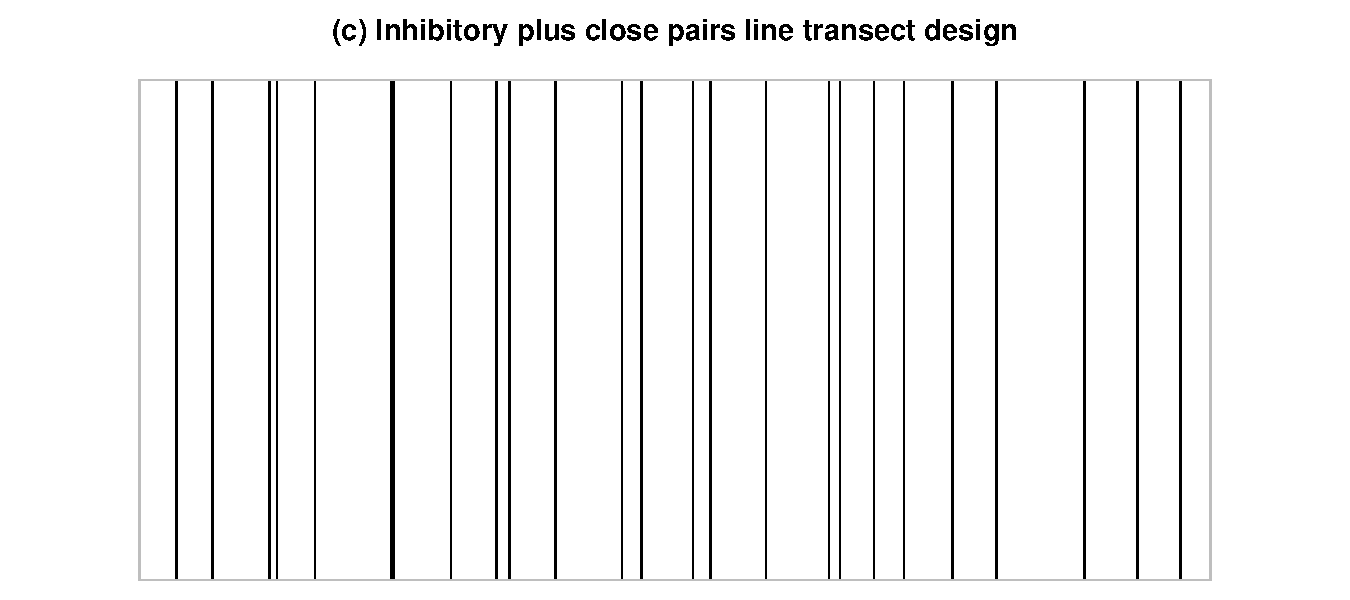
\includegraphics[width=2.5in]{Inhib000171.pdf}
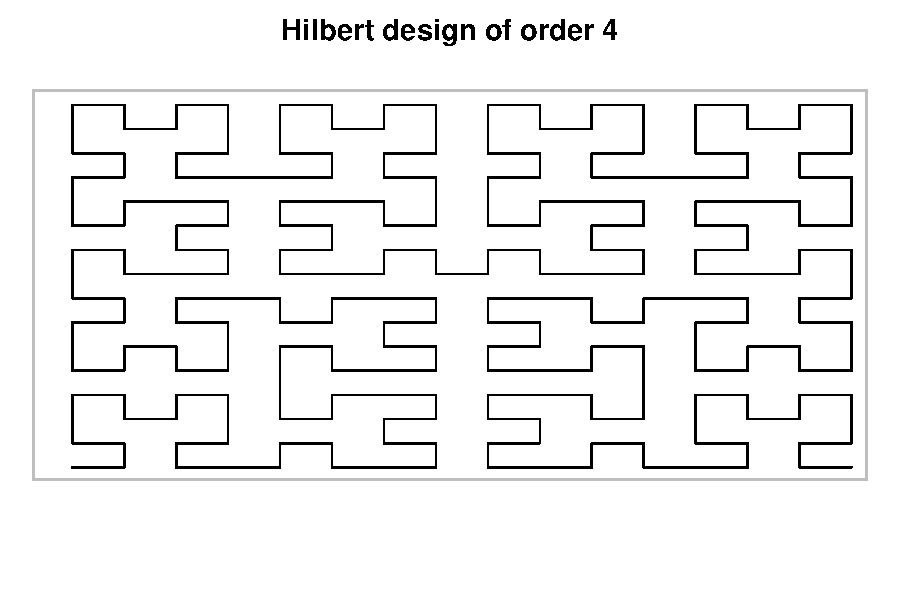
\includegraphics[width=2.5in]{Hilbert000180.pdf}

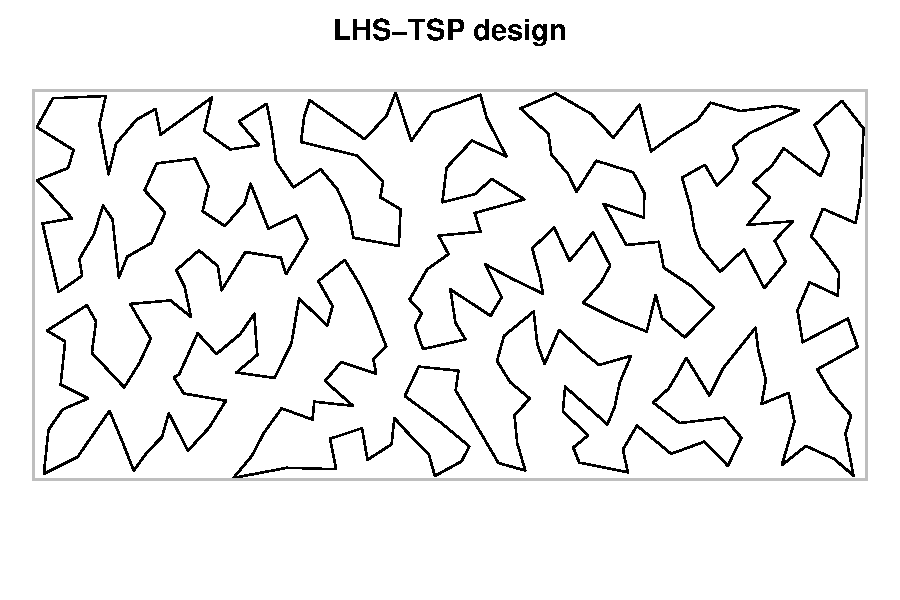
\includegraphics[width=2.5in]{LHS-TSP000161.pdf}
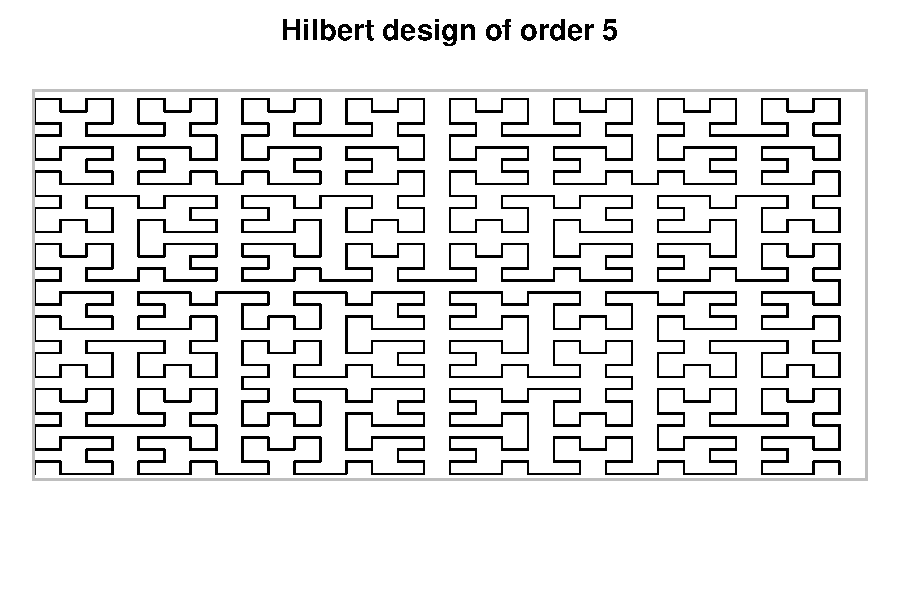
\includegraphics[width=2.5in]{Hilbert000237.pdf}

\caption{Examples of plans from six design schemes. Left, top to bottom: three
different parallel line transect schemes with the same number of transects, and
a shortest path through a Latin hypercube sampling design. Right: two
serpentine transect plans and two Hilbert curves. Except for the Hilbert curve
of order 5, all of these plans have approximately the same total length.}
\label{plancomparison}
\end{figure}


\subsubsection{Parallel serpentine transects}

One simple way to observe a greater variety of locations and different
directions is to add lateral zigzags to transects. We include alternate right
and left turns at right angles to create serpentine transects. This could
decrease prediction variance because more of the path will be close to each
point in the study area than would be under a line transect design with similar
total distance. They will also improve estimation of the covariance function
in the presence of anisotropy. Figure~\ref{plancomparison}, top right, shows
two examples.
% Note: Serp has higher average and max distance from path than Sys but lower
% than SRS and Inhib.

% What to do with the comments about anisotropy? Consolidate them and put them
% in one spot? Anisotropic models are rarely used (underused) and we are
% simulating from isotropic models, but "go in more than one direction if you
% have anisotropic data" is advice worth spending a paragraph on.


\subsubsection{Latin hypercube sampling}

Random Latin hypercube sampling (LHS) produces a design that spreads discrete
points through a (potentially high-dimensional) design space, ensuring that
the full range of each dimension is included while remaining balanced and
keeping the number of points small~\cite{mckayetal}. This is done by
partitioning each dimension into a specified number \(k\) of intervals (thus
stratifying the design space into \(k^{d}\) cells), selecting a Latin
hypercube design to determine which \(k\) cells will contain a design point,
and then drawing each design point from a uniform distribution over its cell.
In two dimensions, this scheme produces point designs with good spatial
coverage properties. We use the LHS design as waypoints for a path. Because
longer distance typically brings increased costs, we treat this as a traveling
salesperson problem (TSP) and use the shortest path through the waypoints as
our design. This LHS-TSP scheme produces paths that have many sharp corners but
leaves few large voids (example in Figure~\ref{plancomparison}, bottom left). A
downside of this design scheme is that the length cannot be specified directly,
and only certain distances are possible depending on the number of bins used.

Waypoints are generated by the \texttt{lhs} R package~\cite{lhs}
and connected into a the shortest path by the \texttt{TSP} package~\citep{tsp}.


\subsubsection{Space-filling curves}

As a representative of space-filling curves, we use the Hilbert curve scaled
to fit the study site. The only parameter of this design scheme is the order,
or number of iterations used in refining the curve. Each iteration increases
the length and complexity of the design. This is produces a deterministic
design, so a random offset is added to vary which points are observed. The
Hilbert curve is generated by \texttt{HilbertVis} R package~\citep{hilbertvis}.

%\paragraph{Particle movement model}
%Models the way data are actually collected. Waypoints generated sequentially by
%generating a jump distance and a direction. The jump distance is generated from
%a scaled beta distribution, and negatively correlated with previous jump
%distance. This behavior should approximately alternate between a short
%``transition'' and a long transect. The negative correlation was achieved by
%applying a \(1 - x\) transformation to a beta autoregressive
%process~\citep{mckenzie}. The direction angle is drawn from a bimodal
%distribution that is symmetric around 0 (a normal distribution reflectd about
%0). {\it explain the Strauss part}

%{\it set up to think about adaptive sampling (adding a transect at a time or
%stopping early but don't actually do it here)}


\subsection{Model fitting}

We fit the spatial LGCP model using nested integrated Laplace approximations
and the R-INLA package~\citep{rueetal,rinla}. The Gaussian process is
approximated using a finite element approach \citep{lindgrenetal}. The point
pattern is modeled by pseudata placed at the events and the finite element
nodes~\citep{simpsonetal}. This procedure allows fast and accurate
approximation of the posterior distribution.%~\citep{flagghoegh}.


\section{Simulation Study}

We simulate 100 designs from each of six schemes. All events within a 2 unit
radius of the path are observed. The whole experiment is repeated for 5
realizations from each of two data generating models.


\subsection{Study site}

We consider a fictitious site \(\mathcal{R}\) with the simple shape of a 1500
unit by 700 unit rectangle. In this site, we will simulate two data generating
models meant to produce random intensity functions with hotspots. First, a LGCP
with latent GP mean \(\mu = \log(250 / |\mathcal{R}|)\) and a Mat\'{e}rn
covariance with \(\nu = 1\), \(\sigma = 2\), and \(\text{range} = 200\). This
model produces relatively unstructured hotspots due to large variability in the
GP.

Second, a two-stage cluster process and a LGCP are superposed. The cluster
process (a Neyman-Scott or, more specifically, a Thomas process) is constructed
as follows. The number of clusters is Poisson with mean 3. The number of events
per cluster is Poisson with mean 200. The cluster centers are distributed
uniformly over \(\mathcal{R}\). Events come from a bivariate normal
distribution with mean equal to the cluster center and variance
\(\boldsymbol{\Sigma} = \tau^{2}\mathbf{I}\), \(\tau = 50\). The LGCP has
\(\mu = \log(250 / |\mathcal{R}|)\) and Mat\'{e}rn covariance with \(\nu = 1\),
\(\sigma = 1\), and \(\text{range} = 200\). This model is based upon the
typical conceptual model of a firing range, with a background process
(represented by the LGCP) and a small number of higher-intensity foreground
clusters containing the events of interest.


\subsection{Path design schemes}

The simulation uses each of the design schemes discussed in
Section~\ref{methodschemes}. The parallel transect schemes have 10,
25, 50, or 70 line transects running north-south. We expect the
simple random sample scheme to produce expect high prediction variance and
large prediction error in big gaps between transects. The systematic sample
scheme uses a uniformly-distributed starting point and constant spacing between
adjacent transects. We expect systematic transects to provide low bias and
moderate prediction variance. However, this scheme can miss structures at
certain sizes because no transects are close to each other in the east-west
direction.

For the inhibitory plus close pairs line transect scheme, we vary the numbers of
paired and unpaired transects. The total number of transects is 10, 25, 50, or
70, with 10\% and 20\% of the transects (rounded to the nearest integer) as
redundant members of a pair. The remaining primary transects are placed
according to a one-dimensional Strauss process \citep{strauss,kellyripley}. The
Strauss attraction parameter is set at \(\gamma = 0.05\) and the radius for
counting pairs is 1500 units divided by the total number of transects. Then
each redundant transect is randomly paired to a primary transect, and placed
within the pair radius of the primary transect according to a uniform
distribution. We expect this scheme to have intermediate performance between
the simple random sample and the systematic line transect schemes.

The serpentine transect scheme has 7, 22, 47, or 67 transects running
north-south with constant east-west spacing and a random starting point for the
first transect. The number of zigzags is 5 or 8, and the zigzag perpedicular
length is set so the the total east-west distance equals the length of three
north-south line transects. Thus, the serpentine designs have the same length
as the line transect designs. These designs should result in smaller
prediction errors and lower variance farther from path, compared to
line-transect designs.

Our Latin hypercube sampling/traveling salesperson (LHS-TSP) scheme uses 50,
300, 1200, or 2400 bins to generate the waypoints. Preliminary experiementation
found that these bin numbers produced total lengths similar to the
line-transect schemes. The LHS-TSP scheme is expected to result in small
prediction errors and low prediction variance per unit distance traveled.
However, the designs will have many sharp corners and may leave some large
voids.

The Hilbert curve scheme uses a random starting point and a Hilbert curve of
order 3, 4, 5, or 6. The path length is a deterministic function of the order
and differs greatly among curves of different orders. These orders yield
lengths similar to the lenths of the transect designs. Hilbert designs should
provide low prediction variance, but have lots of short segments.


\subsection{Model specification}

The same Bayesian LGCP model is fit to each observed dataset. The observed
point pattern \(\mathbf{x}\) is a realization of \(\mathbf{X}\), a Poisson
process on \(\mathcal{R}\) with intensity \(\lambda(u)\). The intensity is
modeled as \(\log[\lambda(u)] = \mu + \mathbf{e}(u)\). The spatial error term
\(\mathbf{e}\) is a Gaussian process with mean \(\mathbf{0}\) and a
Mat\'{e}rn covariance function with fixed \(\nu = 1\).
% Remember alpha = nu + d/2 so alpha = 2 and d = 2 imply nu = 1.

The intercept \(\mu\) has a \(\mathrm{Unif}(-\infty, \infty)\) prior.
% Or \(\mathrm{N}(0, \infty)\)?
The covariance parameters \(\sigma\) and \(\rho\) have a PC prior with
\(\mathrm{Pr}(\sigma > 3) = 0.1\) and \(\mathrm{Pr}(\rho < 100) = 0.1\)
\citep{fuglstadetal,simpsonpc}.

The Gaussian process prediction surface is approximated on the finite element
mesh shown in Figure~\ref{meshfull}.

\begin{figure}
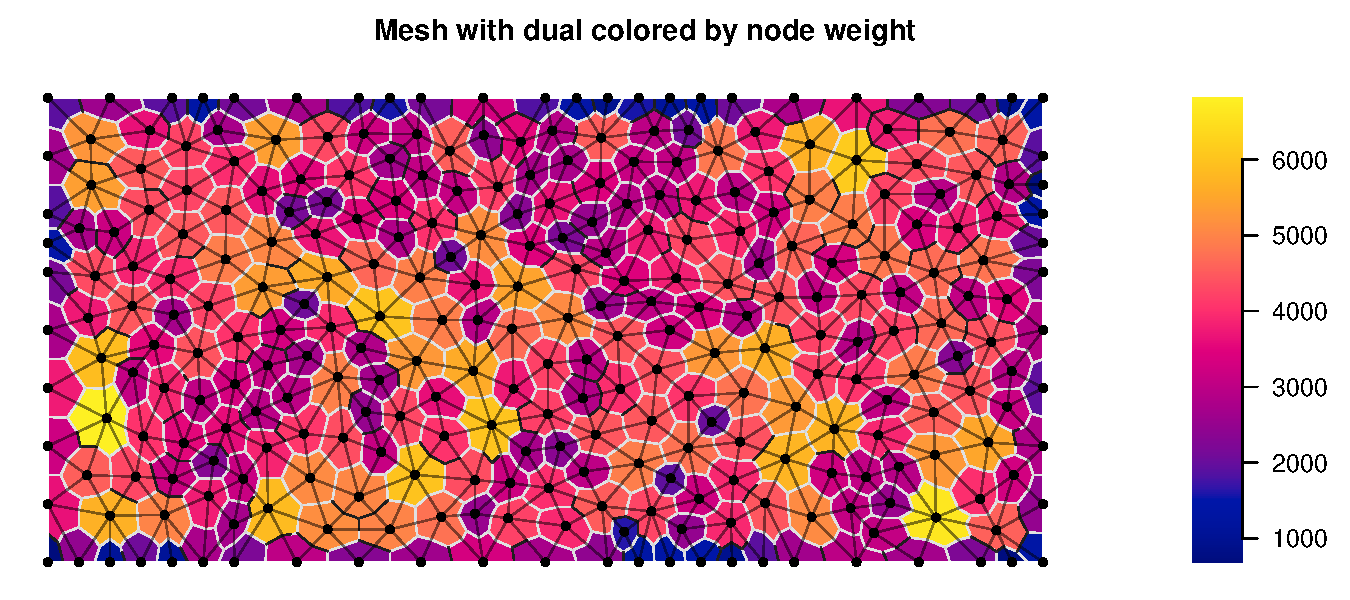
\includegraphics[width=5in]{mesh_full.pdf}
\caption{Illustration of the mesh and associated numerical integration
weighting scheme used to approximate the latent GP.}
\label{meshfull}
\end{figure}


%\section{Theory/calculation}
% A Theory section should extend, not repeat, the background to the article already dealt with in the Introduction and lay the foundation for further work. In contrast, a Calculation section represents a practical development from a theoretical basis.


\section{Results}
% Results should be clear and concise.

%look at examples of designs that minimize each criterion

%look at examples of designs along the Pareto front

%The results section will compare the distribution of prediction variance for
%the Gaussian process averaged over space (APV). We will focus on the average of
%APV for the 100 designs from each scheme applied to each dataset, but will
%point out and discuss if any schemes have large variance or skew in the
%distribution of APV. We will plot the relationships among APV, path length, and
%number of segments. The manuscript will focus on one LGCP dataset and one
%clustered dataset; the analysis of the other datasets will be in the
%supplemenatal materials. The supplemental materials will also include a repeat
%of this analysis for mean squared prediction error (MSPE). The conclusions of
%the MSPE analysis will probably be very similar to those of the APV analysis,
%but if there are any difference will will point them out in the main
%manuscript.

In summarizing the results, we focus on one LGCP dataset and one clustered
dataset (Figure~\ref{fulldata}). Similar patterns were seen for all datasets
(see the online supplement.)

\begin{figure}
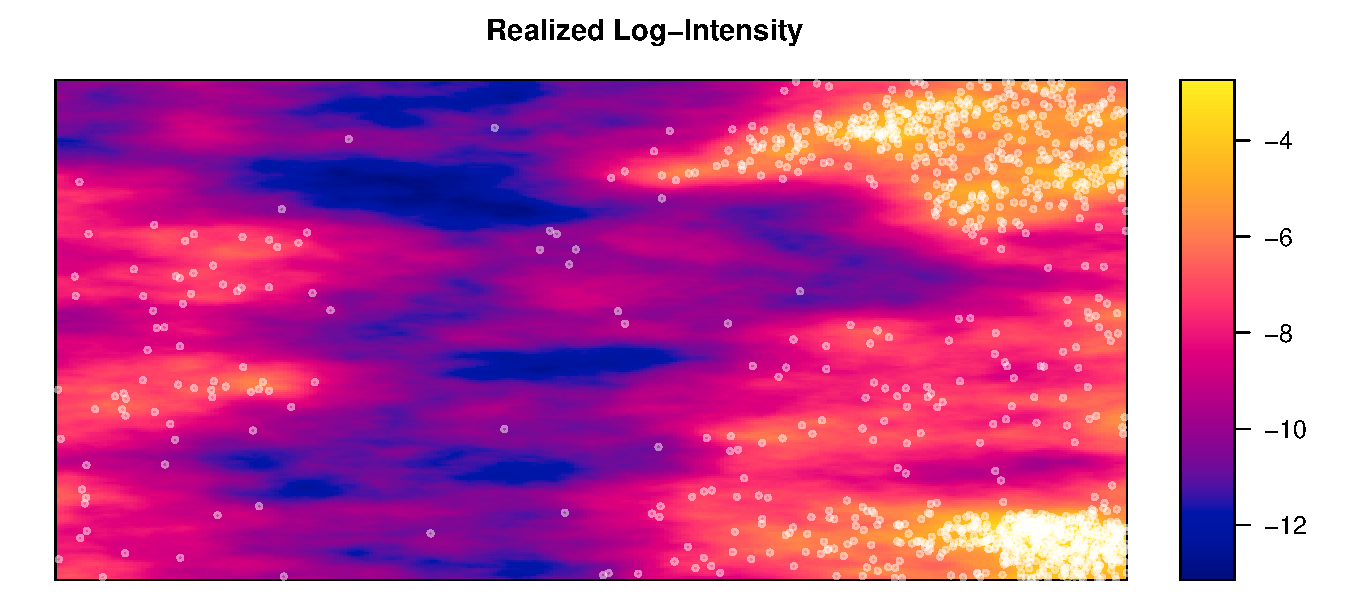
\includegraphics[width=5in]{lambda-LGCP000004.pdf}

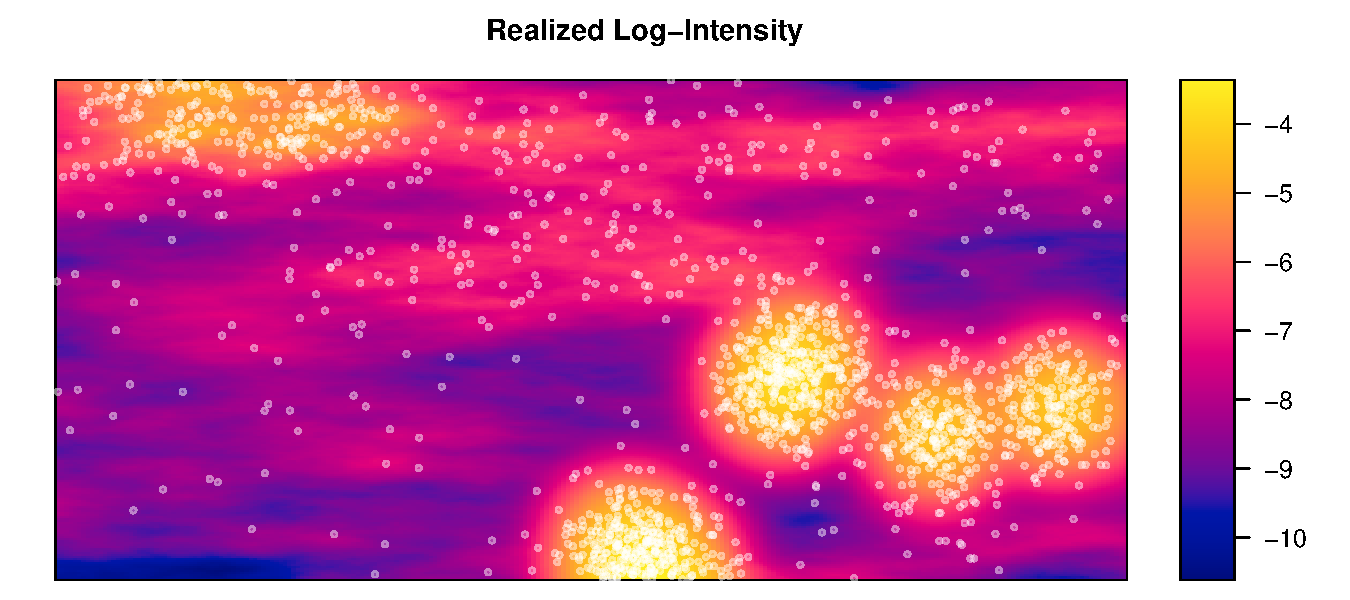
\includegraphics[width=5in]{lambda-Cluster000004.pdf}

\caption{The realized intensity function and complete point pattern from a LGCP
(top) and a LGCP superposed with a cluster process (bottom).}
\label{fulldata}
\end{figure}

big takeways:
\begin{itemize}
\item APV and MSPE both decrease with increasing distance (leveling off at
some point)
\item SD is lowest near obsevered events and increases with distance from
events (not path!), highest at edges of site where there are no events nearby
\item Insubstantial differences among schemes
\begin{itemize}
\item LHS-TSP has lowest median APV for paths under 10000 units but large IQR
\item For longer paths, SRS isn't bad
\item SRS has slightly lower  median and IQR of APV than systematic
\end{itemize}
\item Look at parameter posteriors? Maybe differences within scheme
\item Clusters of high-MSPE
\begin{itemize}
\item Number decrease with distance
\item Associated with certain schemes?
\item Explained by edge effects? Look at more plots
\end{itemize}
\item APV and MSPE not convincingly related
\begin{itemize}
\item Plots vary a lot by dataset
\item Predictions in high-MSPE clusters have high APV but are not outliers
\item Examine spatial prediction surface when evaluating posterior
\end{itemize}
\item Call out a few high and low MSPE example surfaces
\end{itemize}
APV and MSPE both right-skewed. Log all plots. Used median and IQR (or range?)


\section{Discussion}
% This should explore the significance of the results of the work, not repeat them. A combined Results and Discussion section is often appropriate. Avoid extensive citations and discussion of published literature.

%of the schemes considered here, only transect schemes have flexiblility in
%distance and/or a priori known distance

%convergence problems/large variance solution is more data collection?

%discuss starting points for optimization and sequential design

%practical issue: path will be smoothed, no instantaneous direction changes at
%corners, equipment may have limitations which is why we looked at number and
%distribution or turn angles

%could incorporate turns into loss function or use multi-objective
%optimization~\citep{lark}


\section{Conclusions}
% The main conclusions of the study may be presented in a short Conclusions section, which may stand alone or form a subsection of a Discussion or Results and Discussion section.


%\appendix
%\section{Notation and Terminology}

%\begin{itemize}

%\item process defined on \(\mathcal{D} \subset \mathbb{R}^{d}\), domain of the
%intensity function, in this manuscript \(d = 2\)

%\item observation window \(\mathcal{S} \subset \mathcal{D}\)

%\item define three regions:
%\begin{itemize}
%\item the domain \(\mathcal{D}\) over which the process mathematically operates
%\item the study region \(\mathcal{R}\) over which inferences are desired
%\item the observed/sampled observation window \(\mathcal{S}\)
%\end{itemize}

%\item general relationship is \(\mathcal{S} \subset \mathcal{R}
%\subset \mathcal{D} \subset \mathbb{R}^{d}\) where all of the subset symbols
%taken to mean ``subset or equal''

%\item \(\mathcal{D}\) can be bounded or unbounded (often equal to
%\(\mathbb{R}^{d}\)), $\mathcal{S}$ practically always bounded, \(\mathcal{R}\)
%bounded or unbounded depending on application and inferential goals

%\item the ``fully surveyed'' (censused) situation is
%\(\mathcal{S} = \mathcal{R}\)

%\item survey path \(\mathcal{P}\) is a one-dimensional subset of
%\(\mathcal{R}\)
%\begin{itemize}
%\item set of one or more sequences of waypoints connected by line segments
%\item \(\mathcal{S}\) is the set of all points within a fixed (and assumed
%known) radius of \(\mathcal{P}\)
%\end{itemize}

%\item \(\mathbf{X}\) point process on \(\mathcal{R}\), \(\mathbf{x} = \{x_{1},
%\dots, x_{n}\}\) realized point pattern
%\begin{itemize}
%\item \(\mathbf{X}_{\mathcal{S}} = \mathbf{X} \cap \mathcal{S}\) the
% restriction of \(\mathbf{X}\) to \(\mathcal{S}\), \(\mathbf{x} = \mathbf{X}
%\cap \mathcal{S}\) the realized observeable point pattern
%\end{itemize}

%\item point \(x \in \mathbf{x}\) called an event

%\item intensity function \(\lambda(u)\)

%\item types of ``points'' in space:
%\begin{itemize}
%\item \(x\) event in the point pattern
%\item \(s\) numerical integration node
%\item \(u\) arbitrary location in \(\mathcal{D}\) used to index intensity
%function and predictors
%\end{itemize}

%\item \(z(u)\) a column vector of covariates/predictors at \(u\) (not used in
%this manuscript)

%\item ``point'' refers to a \(u\) unless clearly stated otherwise

%\item bold for sets and spatial processes, normal italics for spatial vectors

%\item \(y\) and variations will be used for objects derived from the point
%pattern, e.g. marks, pseudodata

%\item distance sampling fits into the framework with expansion of notation
%to include a (nontrivial) detection function and differentiate between the
%observed and observable point patterns

%\end{itemize}


%\section{Extension of Nearest Neighbor Distance to Paths}


\section*{References}

\bibliography{lgcp_sampling.bib}

\end{document}
